
\documentclass[11pt,a4paper,openany]{report}
\usepackage[T1]{fontenc}
\usepackage[utf8]{inputenc}
\usepackage{lmodern}
\usepackage{microtype}
\usepackage{amsmath,amssymb,amsthm,mathtools,bm}
\usepackage{booktabs,array,longtable,tabularx}
\usepackage{xcolor}
\usepackage[margin=22mm,headheight=23pt]{geometry}
\usepackage{enumitem}
\usepackage{fancyhdr}
\usepackage{fancyvrb}
\usepackage{graphicx}
\usepackage{url}
\usepackage{xurl}
\usepackage{hyperref}
\definecolor{finblue}{HTML}{1F5A99}
\definecolor{fingreen}{HTML}{19733A}
\definecolor{finorange}{HTML}{D55E00}
\definecolor{finred}{HTML}{A61B1B}
\definecolor{finviolet}{HTML}{6A3D9A}
\definecolor{fingray}{HTML}{4D4D4D}

\hypersetup{
  unicode=true,
  colorlinks=true,
  linkcolor=finblue,
  citecolor=fingreen,
  urlcolor=finblue,
  pdftitle={FIN Research Programs P351--P364},
  pdfauthor={Krzysztof Żuchowski},
  pdfsubject={Rigorous moment certificates, graph naturality, operational resource completion, and external physics gates},
  pdfkeywords={FIN, signed moments, Krawczyk method, Bernstein certificate, graph naturality, quantum comb, photonic mesh, resource category, Blaschke factor, operational physics}
}
\pagestyle{fancy}
\fancyhf{}
\fancyhead[L]{\small FIN Programs P351--P364}
\fancyhead[R]{\small Release 10.31}
\fancyfoot[C]{\thepage}

\setlength{\parindent}{0pt}
\setlength{\parskip}{0.55em}
\setlist{nosep,leftmargin=2em}
\setcounter{tocdepth}{2}
\setcounter{secnumdepth}{3}
\emergencystretch=3em
\newcommand{\one}{\bm 1}
\newcommand{\C}{\mathbb C}
\newcommand{\R}{\mathbb R}
\newcommand{\Z}{\mathbb Z}
\newcommand{\statusProven}{\textcolor{fingreen}{[Proven]}}
\newcommand{\statusStrong}{\textcolor{finblue}{[Strong evidence]}}
\newcommand{\statusModerate}{\textcolor{finviolet}{[Moderate evidence]}}
\newcommand{\statusWeak}{\textcolor{fingray}{[Weak evidence]}}
\newcommand{\statusSpeculative}{\textcolor{finorange}{[Speculative]}}
\newcommand{\statusRefuted}{\textcolor{finred}{[Refuted]}}

\begin{document}
\hypersetup{pageanchor=false}
\begin{titlepage}
\centering
\vspace*{7mm}
{\Large\bfseries FIN --- Release 10.31\par}
\vspace{9mm}
{\Huge\bfseries Research Programs P351--P364\par}
\vspace{6mm}
{\Large Rigorous moment certificates, graph naturality,\\
operational resource completion, and external physics gates\par}
\vspace{13mm}
{\Large Krzysztof \.Zuchowski\par}
\vspace{2mm}
{\normalsize Independent Researcher --- Fractal Information Theory Project\par}
\vspace{2mm}
{\normalsize ORCID:
\href{https://orcid.org/0009-0002-0909-3613}{0009-0002-0909-3613}\par}
\vspace{7mm}
{\large 31 July 2026\par}
{\normalsize Publication --- Preprint; Version 1.0.0\par}
\vfill
\begin{minipage}{0.92\textwidth}
\small
\textbf{Certified attenuation resource.}
\[
0.4067063265581317
\leq\mathcal N_{\rm env}
\leq0.4067063346922584.
\]

\textbf{Certified oscillatory resource.}
\[
0.7072782253162320
\leq\mathcal N_{\rm osc}
\leq0.7073599748862595.
\]

Both are classical signed-representation costs. No physical-negativity,
information-loss, selector, unit, role-transfer, laboratory, total-action,
Standard-Model, gravity, or Theory-of-Everything closure is claimed.

\medskip
\textbf{Repository.}
\url{https://github.com/hyconiek/Fractal-Nadsoliton-Theory}

\textbf{License.} CC BY 4.0.
\end{minipage}
\vfill
\end{titlepage}
\hypersetup{pageanchor=true}
\pagenumbering{roman}
\chapter*{Publication statement}
\addcontentsline{toc}{chapter}{Publication statement}
This monograph reports every executed Program P351--P364 and recommends
Programs P365--P378. Exact proof, strong numerical evidence, synthetic
apparatus design, conditional physics, and missing external evidence are
kept distinct. The legacy/strict split and all current strict-core
guardrails remain binding.

\tableofcontents
\clearpage
\pagenumbering{arabic}

\chapter*{Confidence convention}
\addcontentsline{toc}{chapter}{Confidence convention}

\begin{center}
\begingroup\small
\setlength{\tabcolsep}{2.5pt}
\renewcommand{\arraystretch}{1.16}
\begin{longtable}{@{}p{0.420\textwidth}p{0.420\textwidth}@{}}
\toprule
\textbf{Label} & \textbf{Meaning in this report} \\
\midrule
\endhead
\textbf{\statusProven{}} & Exact mathematical proof, exact rational finite computation, or compiled structural formal theorem \\
\textbf{\statusStrong{}} & Stable high-precision computation with explicit residual and falsification boundary \\
\textbf{\statusModerate{}} & Reproducible model-based result whose interpretation depends materially on declared assumptions \\
\textbf{\statusSpeculative{}} & A proposed research route without a completed witness \\
\textbf{\statusRefuted{}} & The stated construction fails in its declared class \\
\textbf{[Blocked by external evidence]} & Independent data, custody, hardware, calibration, or unblinding is required \\
\textbf{[Conditional]} & The conclusion follows only after named additional axioms or standards are supplied \\
\bottomrule
\end{longtable}
\endgroup
\end{center}

\chapter{Scope and scientific guardrails}

\section{Kernel split}

The two kernels remain distinct:

\[
K_{\mathrm{legacy,ont}}(d)=
4\ln2\,
\frac{\cos(\pi d/4+\pi/6)}{1+0.01d},
\]

and

\[
K_{\mathrm{strict,gate}}(d)=
\frac{\cos((743/4000)d+13/80)}{1+d^{9/5}}.
\]

The legacy kernel is an intermediate bridge kernel. The strict kernel is the later enriched working object. An identity between them is not assumed. Historical assignments involving \(\sin^2\theta_W\), the electromagnetic coupling, or a gravitational hierarchy are not transferred.

\section{Ontological boundary}

The repository's internal order is recorded as

\[
\text{nadsoliton}
\longrightarrow \text{light}
\longrightarrow \text{matter}
\longrightarrow \text{emergent observer}.
\]

The nadsoliton is described internally as primordial fractal information in a solitonic state, not as an object sitting above a lower informational layer. This report neither proves nor uses that interpretation in its mathematical theorems.

\section{Open strict boundaries}

The following are not closed:

\begin{itemize}
\item 
the non-premise selector and QW-2191;

\item 
a source-independent legacy-to-strict completion theorem;

\item 
a role-transfer theorem;

\item 
an internally generated dimensional standard;

\item 
an experimentally realized preparation/\allowbreak{}channel/\allowbreak{}instrument/\allowbreak{}record system;

\item 
a unit-bearing nonproxy total action;

\item 
Standard Model or gravity derivation;

\item 
Theory-of-Everything closure.

\end{itemize}

\section{Why this research round is noncyclic}

Programs P351--P364 do not rename an existing obstruction. They introduce five genuinely new proof objects:

\begin{enumerate}
\item 
a rational Krawczyk cell;

\item 
a rational oscillatory primal-dual interval;

\item 
a graph-morphism naturality theorem with an explicit counterexample;

\item 
a perfect-comb collapse certificate;

\item 
an inner-factor phase torsor and a typed operational resource category.

\end{enumerate}

External programs are executed only as admission gates. Their failure to admit evidence is reported as a boundary, not as negative experimental data.

\chapter{Executive result table}

\begin{center}
\begingroup\small
\setlength{\tabcolsep}{2.5pt}
\renewcommand{\arraystretch}{1.16}
\begin{longtable}{@{}p{0.152\textwidth}p{0.420\textwidth}p{0.288\textwidth}@{}}
\toprule
\textbf{Program} & \textbf{Main result} & \textbf{Status} \\
\midrule
\endhead
P351 & Exact Krawczyk primal certificate and global optimum enclosure for the attenuation moments & \statusProven{} \\
P352 & Exact rational primal-dual enclosure for the full oscillatory moments & \statusProven{} \\
P353 & No independently frozen QW hold-out bundle admitted & [Blocked] \\
P354 & Radial-kernel naturality for isomorphisms; homomorphism counterexample & \statusProven{} /\allowbreak{} \statusRefuted{} \\
P355 & Loss-aware synthetic twelve-mode compiled-mesh digital twin & \statusModerate{} \\
P356 & No calibrated physical photonic bundle admitted & [Blocked] \\
P357 & Full-comb optimality theorem at convex-zero witnesses; four FIN instances & \statusProven{} /\allowbreak{} \statusStrong{} \\
P358 & Equispaced minimax bounded-curvature clock design after an external anchor & \statusProven{} \\
P359 & Complete cancellative five-resource preorder; no catalysis & \statusProven{} in declared category \\
P360 & Analytic inner-factor obstruction to amplitude-to-phase recovery & \statusProven{} /\allowbreak{} \statusRefuted{} \\
P361 & No blinded conditional electroweak record admitted & [Blocked] \\
P362 & Exact conversion-frame covariance pushforward; no standards admitted & \statusProven{} /\allowbreak{} [Blocked] \\
P363 & Minimal FIN Operational Resource Completion category & \statusProven{} relative construction \\
P364 & No calibrated physical-reservoir execution admitted & [Blocked] \\
\bottomrule
\end{longtable}
\endgroup
\end{center}

\chapter{Mathematical preliminaries}

\section{Signed Hausdorff moment cost}

For a finite real sequence \(m_0,\ldots,m_q\), define

\[
\mathcal N(m)=
\inf_{\mu}
\mu^-([0,1]),
\]

where \(\mu=\mu^+-\mu^-\) is a finite signed measure satisfying

\[
\int_0^1 x^n\,d\mu(x)=m_n,
\qquad n=0,\ldots,q.
\]

The dual problem uses

\[
p(x)=\sum_{n=0}^{q}a_nx^n,
\qquad -1\leq p(x)\leq0,
\]

and gives

\[
\sum_{n=0}^{q}a_nm_n
\leq \mathcal N(m).
\]

This follows because

\[
\int p\,d\mu
=\int p\,d\mu^+-\int p\,d\mu^-
\leq \mu^-([0,1]).
\]

A dual polynomial therefore supplies a lower bound, while any explicit signed representing measure supplies an upper bound.

\section{Exact interval arithmetic}

Every interval endpoint used in P351 and P352 is rational. Arithmetic uses the inclusion rules

\[
[a,b]+[c,d]=[a+c,b+d],
\]

\[
[a,b][c,d]=
\left[
\min(ac,ad,bc,bd),
\max(ac,ad,bc,bd)
\right].
\]

For \(n>0\), a rational bracket of \(n^{1/5}\) is obtained by integer arithmetic:

\[
r_-^5\leq n\leq r_+^5.
\]

It follows that

\[
\frac{1}{1+r_+^9}
\leq
\frac{1}{1+n^{9/5}}
\leq
\frac{1}{1+r_-^9}.
\]

No floating-point evaluation is used to justify the inclusion.

\section{Compact identities for large rationals}

Some exact Krawczyk endpoints contain more than ten thousand binary digits. Printing them in a scientific table would make the report less auditable. The CSV therefore records:

\begin{itemize}
\item 
numerator bit length;

\item 
denominator bit length;

\item 
a SHA-256 identity of sign, numerator bytes, and denominator bytes;

\item 
a decimal projection for reading.

\end{itemize}

The executable source recomputes each exact rational. The digest is an identity check, not a replacement for the calculation.

\chapter{P351 --- exact primal certification of the attenuation resource}

\section{Moment system}

P323 represented the six positive-order moments using three positive atoms:

\[
\sum_{i=1}^{3}u_ir_i^n=h_n,
\qquad n=1,\ldots,6.
\]

The approximate centers are

\[
\begin{aligned}
r_1&\approx0.2372783418730673,\\
r_2&\approx0.5481980169862998,\\
r_3&\approx0.8527659803199023,
\end{aligned}
\]

and

\[
\begin{aligned}
u_1&\approx0.9418342033805291,\\
u_2&\approx0.3936855195357094,\\
u_3&\approx0.0711866117760197.
\end{aligned}
\]

The missing zeroth moment is supplied by

\[
-N\delta_0,
\qquad
N=u_1+u_2+u_3-1.
\]

\section{Krawczyk operator}

Let \(x=(r_1,r_2,r_3,u_1,u_2,u_3)\) and let \(F(x)\) contain the six moment residuals. For a rational box \(X\), rational center \(x_0\), and rational approximate inverse \(C\) of \(DF(x_0)\), define

\[
\mathcal K(X)=
x_0-CF(x_0)+
\left(I-C\,DF(X)\right)(X-x_0).
\]

P351 uses radius \(10^{-12}\) in all six coordinates and interval moments with sixty decimal digits in the fifth-root brackets.

The exact computation proves

\[
\mathcal K(X)\subset\operatorname{int}(X).
\]

Therefore \(F\) has exactly one zero in \(X\). The entire box lies in

\[
0<r_1<r_2<r_3<1,
\qquad
u_i>0.
\]

\section{Global enclosure}

The Krawczyk image encloses a feasible primal signed measure. Combining its upper mass with the exact P337 rational dual gives

\[
\boxed{
0.4067063265581317
\leq \mathcal N_{\mathrm{env}}
\leq 0.4067063346922584
}.
\]

The width is

\[
8.134126653281584\times10^{-9}.
\]

\section{What is proved}

\textbf{\statusProven{}}

\begin{itemize}
\item 
existence of a positive ordered three-atom solution in the stated box;

\item 
uniqueness of that solution inside the box;

\item 
feasibility of the associated signed measure;

\item 
the global primal-dual enclosure above.

\end{itemize}

\section{What is not proved}

The Krawczyk result does not prove:

\begin{itemize}
\item 
that this signed measure is a quantum quasiprobability;

\item 
that negative mass is lost information;

\item 
that \(N\) is energy, entropy, action, or a coupling constant;

\item 
that the three atoms have a selected physical realization.

\end{itemize}

The resource is a mathematical obstruction to positive representability.

\begin{figure}[htbp]
\centering
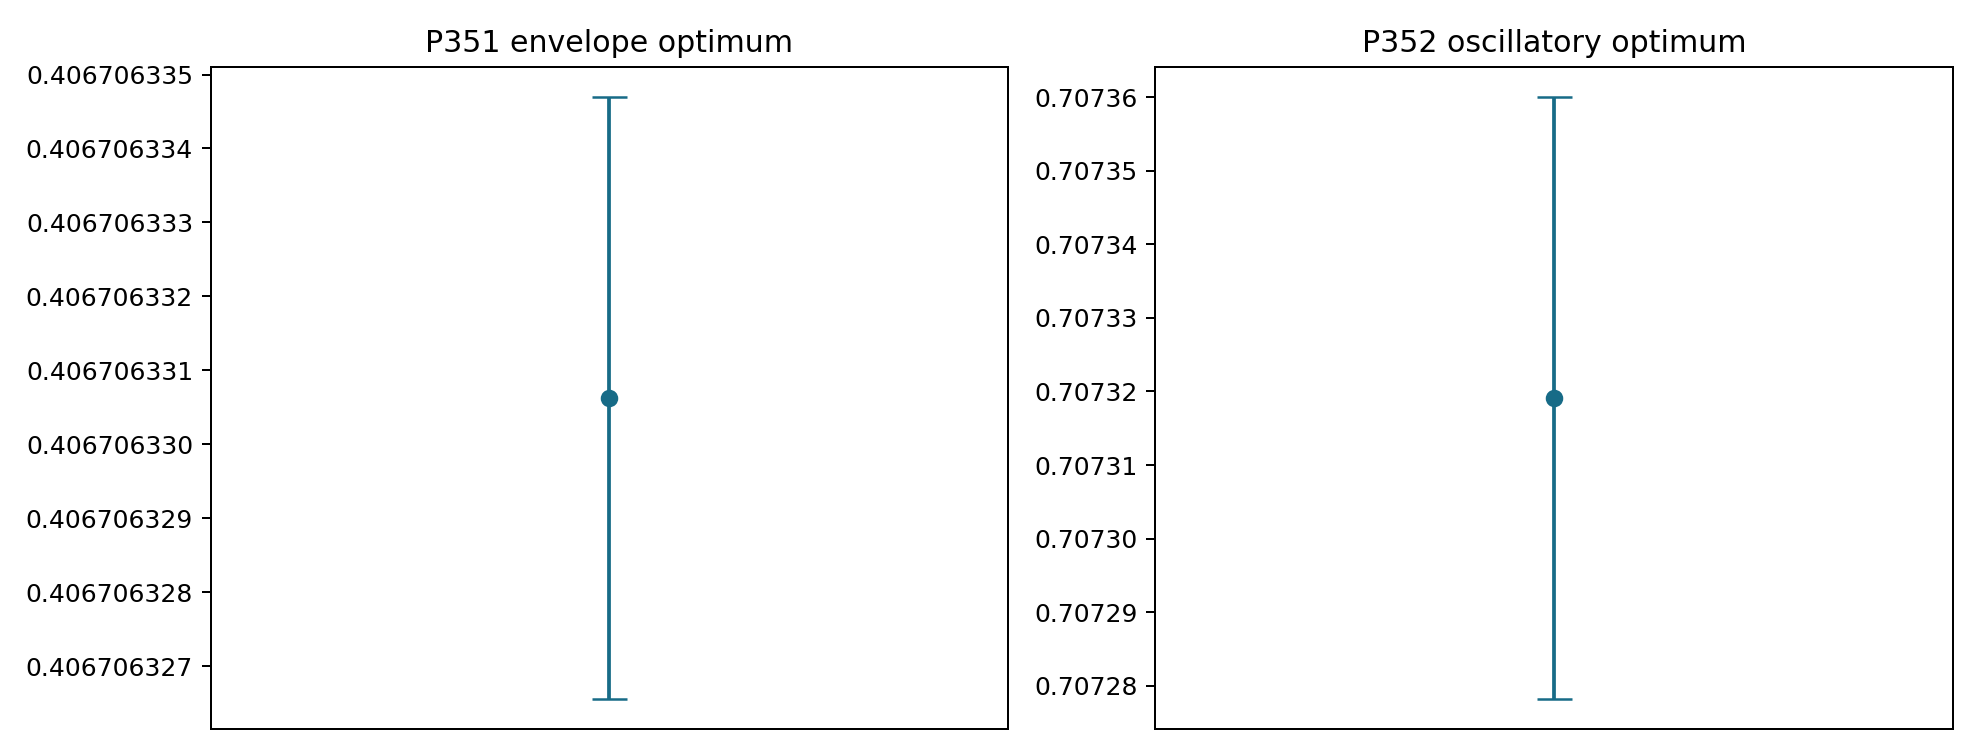
\includegraphics[width=0.97\textwidth]{FIN_Programs_351_364_Figures/p351_p352_rigorous_enclosures.png}
\caption{The theorem-grade primal-dual enclosures for the attenuation and full oscillatory signed-moment resources.}
\end{figure}

\chapter{P352 --- theorem-grade full oscillatory resource}

\section{Target sequence}

The full strict sequence contains both damping and phase:

\[
k_n=
\frac{\cos(\omega n+\phi)}{1+n^{9/5}},
\qquad
\omega=\frac{743}{4000},
\quad
\phi=\frac{13}{80}.
\]

The moments \(k_8,k_9,k_{10},k_{11}\) are negative. A positive measure on \([0,1]\) is therefore impossible immediately, but the minimum signed cost is not determined by the sign test alone.

\section{Rigorous trigonometric enclosure}

For rational \(x\), P352 evaluates

\[
\cos x=
\sum_{j=0}^{M}
(-1)^j\frac{x^{2j}}{(2j)!}+R_M(x),
\]

with

\[
|R_M(x)|
\leq
\frac{|x|^{2M+2}}{(2M+2)!}.
\]

The calculation uses \(M=42\). Combining this with exact fifth-root brackets produces rational intervals for all twelve \(k_n\).

\section{Exact dual feasibility}

The numerically discovered degree-eleven polynomial is converted to rational coefficients. Exact Bernstein subdivision on 4096 rational subintervals produces a global enclosure \([L,U]\). The affine normalization

\[
p_{\mathrm{safe}}(x)=
\frac{p_{\mathrm{raw}}(x)-U}{U-L}
\]

then has exact Bernstein range contained in

\[
-1\leq p_{\mathrm{safe}}(x)\leq0
\qquad (0\leq x\leq1).
\]

This converts the former numerical critical-point check into a global exact dual certificate.

\section{Exact fixed-support primal}

The twelve rational support points are

\[
\frac{79}{4000},\frac{80}{4000},
\frac{517}{4000},\frac{518}{4000},
\frac{1180}{4000},\frac{1181}{4000},
\frac{2107}{4000},
\frac{3256}{4000},\frac{3257}{4000},
\frac{3767}{4000},\frac{3768}{4000},1.
\]

Let \(V_{ni}=x_i^n\). Since these nodes are distinct, \(V\) is invertible. P352 computes \(V^{-1}\) exactly over the rationals and applies it to the moment intervals:

\[
w=V^{-1}k.
\]

Every resulting weight interval excludes zero. Eight weights are positive and four negative. Thus the true moment vector has an exactly feasible signed measure on this support with a certified negative mass.

\section{Result}

\[
\boxed{
0.7072782253162320
\leq \mathcal N_{\mathrm{osc}}
\leq 0.7073599748862595
}.
\]

The width is

\[
8.174957002754137\times10^{-5}.
\]

The earlier P338 lower value is slightly sharper numerically, but P352's lower endpoint is the theorem-grade endpoint after exact safety normalization.

\section{Falsification boundary}

The result falsifies the claim that the full strict sequence is generated by a positive scalar path mixture on \([0,1]\). It does not distinguish among:

\begin{itemize}
\item 
a classical signed path expansion;

\item 
an amplitude-level interference representation;

\item 
a dilation on a larger positive state space;

\item 
a quantum quasiprobability;

\item 
an effective subtraction induced by conditioning.

\end{itemize}

Those interpretations require different operational data.

\chapter{P353 --- independent hold-out admission gate}

\section{Admission contract}

A valid hold-out manifest must contain:

\begin{itemize}
\item 
provider;

\item 
registrar;

\item 
analyst;

\item 
frozen dataset hash;

\item 
freeze timestamp;

\item 
unblinding authorization.

\end{itemize}

The three roles must be distinct. Synthetic, template, and example artifacts are inadmissible.

\section{Result}

No candidate manifest satisfying the contract was found.

\textbf{[Blocked by external evidence]}

This means only that external validation has not occurred. It does not invalidate the internal QW calculation, and it does not convert the in-sample fit into a prediction.

\chapter{P354 --- the categorical naturality boundary}

\section{Graph-isomorphism theorem}

Let \(G\) be a finite connected graph with distance \(d_G\) and radial law \(k:\mathbb N\to\mathbb R\). Define

\[
K_G(x,y)=
\begin{cases}
k(d_G(x,y)),&x\ne y,\\
0,&x=y.
\end{cases}
\]

For a graph isomorphism \(f:G\to H\),

\[
d_H(f(x),f(y))=d_G(x,y).
\]

Therefore

\[
K_H(f(x),f(y))=K_G(x,y).
\]

In matrix form, if \(P_f\) is the permutation matrix,

\[
K_H=P_fK_GP_f^\top.
\]

This is an exact naturality theorem for the groupoid of finite connected graphs and graph isomorphisms.

\section{Homomorphism obstruction}

A graph homomorphism preserves adjacency but may shorten distances. Consider the identity vertex map

\[
P_3\longrightarrow K_3.
\]

The two endpoints have source distance two and target distance one. For the strict radial law,

\[
|k_{\mathrm{strict}}(2)-k_{\mathrm{strict}}(1)|
=0.2779421209549173.
\]

Thus unrestricted graph-homomorphism naturality fails.

\section{Consequence for completion maps}

A legacy-to-strict completion may be natural on:

\begin{itemize}
\item 
graph isomorphisms;

\item 
distance-preserving embeddings;

\item 
an enriched category carrying a declared metric transport.

\end{itemize}

It is not automatically natural on arbitrary graph homomorphisms. Moreover, the C12 scalar spectral interpolant from P340 fails on noncycle carriers. Commutation on C12 is necessary for a scalar functional calculus but not sufficient for carrier-natural completion.

\section{New object}

\textbf{O104 --- Distance-Functor Naturality Boundary}

This object records:

\[
(\text{carrier category},
\text{distance transport},
\text{kernel transport defect}).
\]

It prevents a formula reused on several carriers from being mistaken for a categorical law.

\chapter{P355--P356 --- photonic digital twin and hardware gate}

\section{Compiled target}

At the declared witness time, the strict wave propagator

\[
U_t=e^{-itA_{\mathrm{strict}}}
\]

admits a 66-rotation Givens decomposition in twelve modes.

\section{Loss/\allowbreak{}noise model}

P355 applies:

\begin{itemize}
\item 
\(10^{-4}\)-radian mesh quantization;

\item 
mode-diagonal attenuation accumulated by Givens participation;

\item 
loss settings from \(0\) to \(0.01\) dB per participation;

\item 
output phase noise from \(0\) to \(10^{-3}\) radians;

\item 
\(0.2\%\) multiplicative efficiency-calibration error;

\item 
64 synthetic repetitions per setting.

\end{itemize}

The measured conditional vertex probabilities are

\[
\widehat p(y|x,\mathrm{click})
=
\frac{|T_{yx}|^2}
{\sum_z|T_{zx}|^2}.
\]

Calibration divides out the estimated output efficiencies before renormalization.

\section{Result}

The largest tested 95th-percentile corrected vertex total-variation defect is

\[
1.5953851724811012\times10^{-3}.
\]

\textbf{\statusModerate{}}

The result shows that the declared diagonal-loss model is compatible with millipercent-scale conditional-distribution recovery.

\section{Model destruction tests}

The calculation intentionally does not absorb:

\begin{itemize}
\item 
correlated interferometer fabrication errors;

\item 
phase-dependent loss inside every beam splitter;

\item 
thermal drift;

\item 
source multiphoton contamination;

\item 
detector dead time and afterpulsing;

\item 
time-dependent calibration;

\item 
a mismatch between the intended and fabricated graph.

\end{itemize}

Any one of these may dominate the simulated error. Therefore the digital twin is not a feasibility theorem for a laboratory.

\section{P356 admission result}

No hardware manifest containing independent custody, raw-record hash, calibration hash, freeze timestamp, and unblinding authorization was admitted.

\textbf{[Blocked by external evidence]}

\begin{figure}[htbp]
\centering
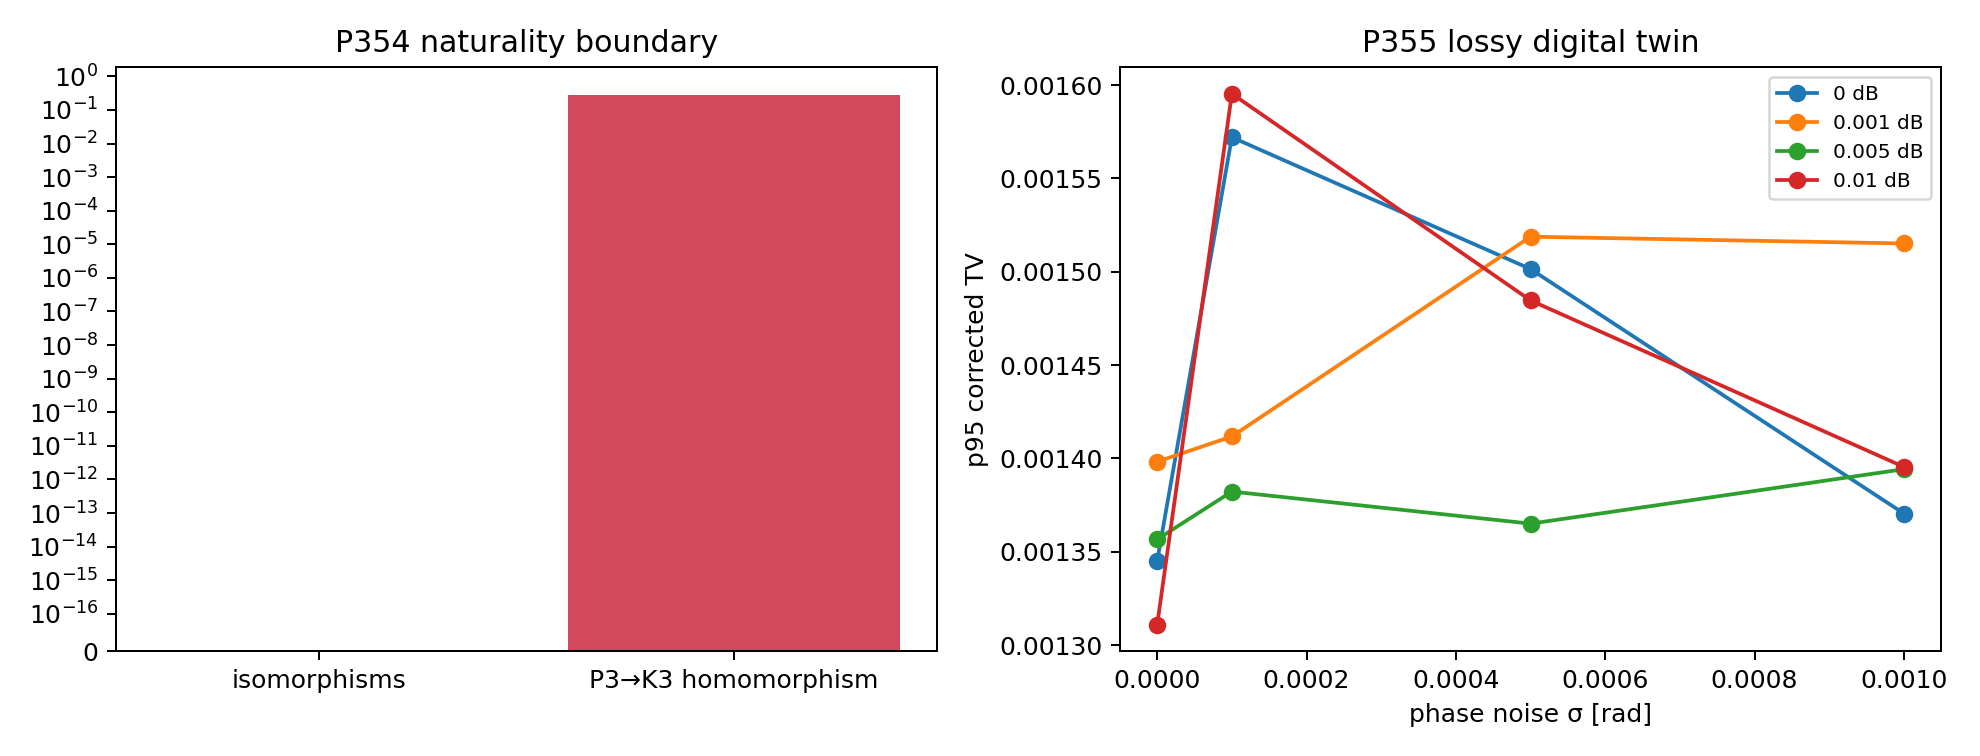
\includegraphics[width=0.97\textwidth]{FIN_Programs_351_364_Figures/p354_p355_naturality_loss.png}
\caption{The exact graph-morphism naturality boundary and the declared loss-aware photonic digital twin.}
\end{figure}

\chapter{P357 --- when a parallel witness solves the full adaptive comb}

\section{Relative-unitary reduction}

For two unitary channels with relative unitary

\[
V=U_{\mathrm{strict}}^\dagger U_{\mathrm{legacy}},
\]

let \(z_j\) be the eigenvalues of \(V\). For \(n\) parallel uses, the relative eigenvalues are products

\[
z_{\mathbf j}=z_{j_1}\cdots z_{j_n}.
\]

Choose a pure input with probability weights \(\lambda_{\mathbf j}\) in the joint relative-eigenbasis. The overlap of the two output states is

\[
\langle\psi_{\mathrm{strict}}|
\psi_{\mathrm{legacy}}\rangle
=
\sum_{\mathbf j}\lambda_{\mathbf j}z_{\mathbf j}.
\]

\section{Perfect-comb collapse theorem}

If

\[
\lambda_{\mathbf j}\geq0,\qquad
\sum_{\mathbf j}\lambda_{\mathbf j}=1,\qquad
\sum_{\mathbf j}\lambda_{\mathbf j}z_{\mathbf j}=0,
\]

then the two output states are orthogonal. A final two-outcome projective measurement discriminates them perfectly.

Every adaptive quantum comb has output trace distance at most two. The parallel strategy achieves two. Hence it is globally optimal even among unrestricted adaptive strategies.

This conclusion does not require proving that adaptivity is never useful. It uses the universal upper bound only at a point where a parallel strategy saturates it.

\section{FIN witnesses}

\begin{center}
\begingroup\small
\setlength{\tabcolsep}{2.5pt}
\renewcommand{\arraystretch}{1.16}
\begin{longtable}{@{}p{0.106\textwidth}p{0.134\textwidth}p{0.201\textwidth}p{0.420\textwidth}@{}}
\toprule
\textbf{Uses} & \textbf{Time per use} & \textbf{Active joint modes} & \textbf{Convex-zero residual} \\
\midrule
\endhead
1 & 0.72 & 3 & \(1.18\times10^{-16}\) \\
2 & 0.36 & 3 & \(5.54\times10^{-16}\) \\
3 & 0.24 & 3 & \(0\) at displayed precision \\
4 & 0.18 & 3 & \(2.22\times10^{-16}\) \\
\bottomrule
\end{longtable}
\endgroup
\end{center}

The structural theorem is \textbf{\statusProven{}}. The four FIN zero-barycenter instances are \textbf{\statusStrong{}} because the phases and barycenters are evaluated numerically rather than enclosed by interval phase arithmetic.

\section{Open subcritical problem}

For times below the first perfect witness, the full adaptive-comb optimum is not obtained from saturation. A primal-dual comb semidefinite program or an analytic commuting-unitary theorem is still required.

\chapter{P358 --- anchored bounded-curvature time}

\section{Clock class}

Assume

\[
\tau(0)=0,\qquad
\tau'(t)>0,\qquad
|\tau''(t)|\leq M=0.2
\]

on \([0,T]\) with \(T=1.4\). A calibrated external value is still needed to define the dimensional scale.

\section{Maximum-gap theorem}

Any design dividing \([0,T]\) into \(m\) intervals has

\[
h_{\max}\geq\frac{T}{m}.
\]

Equality holds for equal spacing. For linear interpolation of a twice-differentiable clock,

\[
\|\tau-\tau_{\mathrm{lin}}\|_\infty
\leq \frac{M h_{\max}^2}{8}.
\]

Therefore equispacing minimizes this worst-case upper bound.

\section{Sample count}

To guarantee error at most \(\varepsilon\),

\[
m\geq
\left\lceil
T\sqrt{\frac{M}{8\varepsilon}}
\right\rceil.
\]

For \(\varepsilon=10^{-3}\),

\[
m_{\min}=7.
\]

This is a theorem about placement after a time standard is supplied. It does not derive time from a dimensionless operator.

\begin{figure}[htbp]
\centering
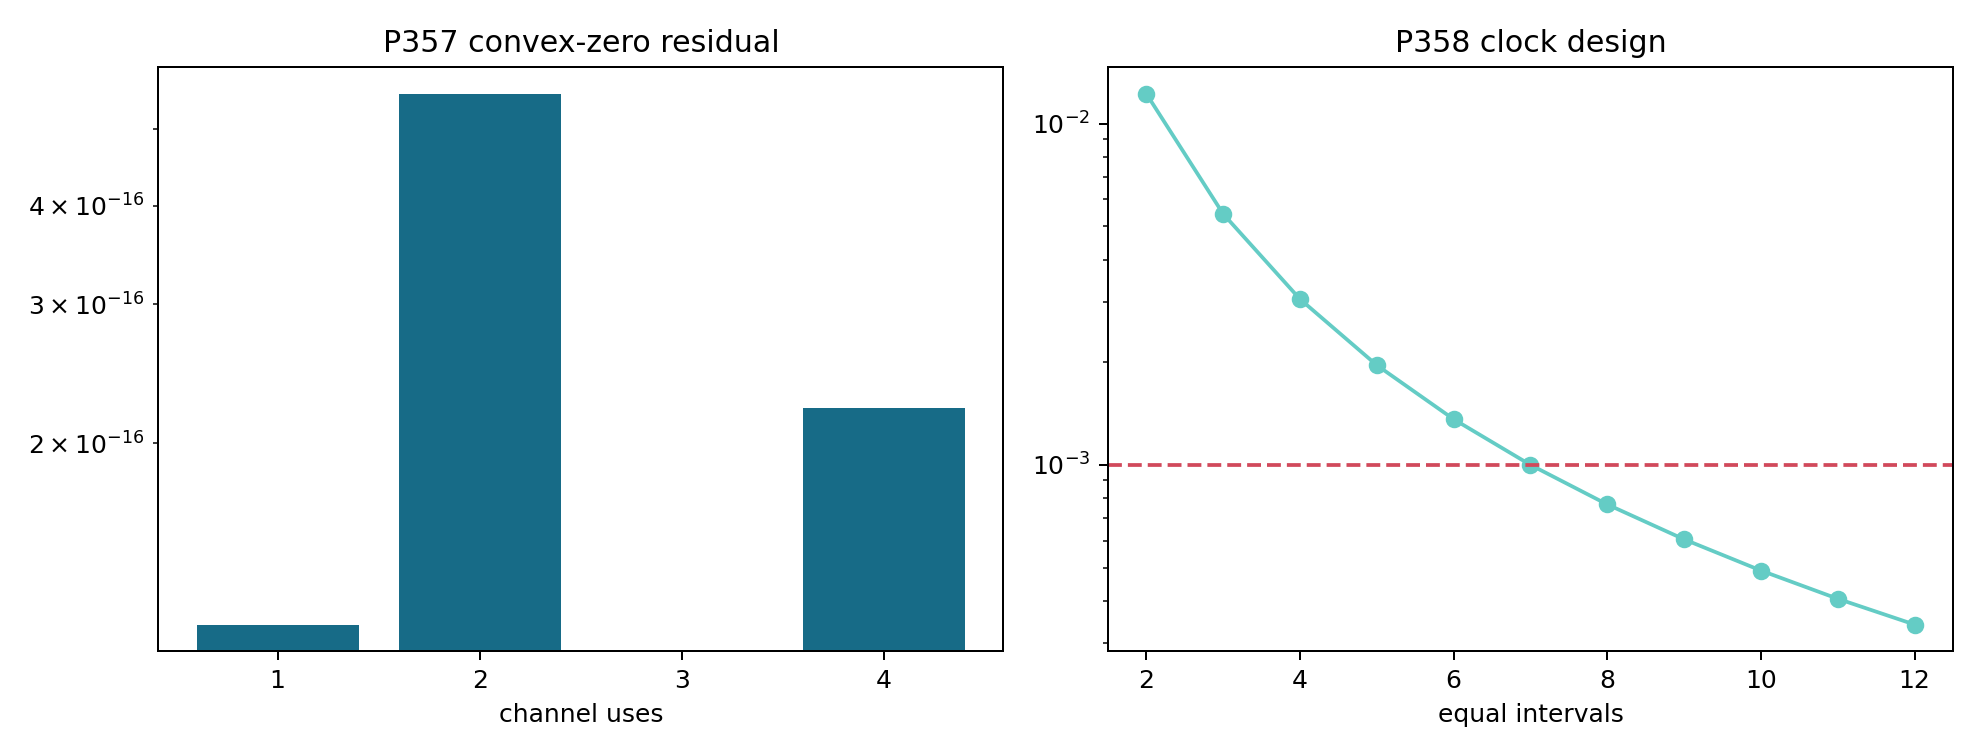
\includegraphics[width=0.97\textwidth]{FIN_Programs_351_364_Figures/p357_p358_comb_clock.png}
\caption{Convex-zero multi-use channel witnesses and the bounded-curvature clock-design envelope.}
\end{figure}

\chapter{P359 --- complete bridge-resource monotones}

\section{Resource object}

Define the resource vector

\[
r=(r_{\mathrm{sign}},
r_{\mathrm{phase}},
r_{\mathrm{orient}},
r_{\mathrm{scale}},
r_{\mathrm{cross}})
\in\mathbb N^5.
\]

The coordinates respectively count:

\begin{enumerate}
\item 
signed-path resource;

\item 
non-torsion phase resource;

\item 
pointing/\allowbreak{}orientation resource;

\item 
positive dimensional-scale resource;

\item 
independent cross-law resource.

\end{enumerate}

\section{Free conversions}

The declared free preorder is

\[
r\longrightarrow s
\quad\Longleftrightarrow\quad
r_i\geq s_i\quad\text{for all }i.
\]

Parallel composition is addition:

\[
r\otimes s=r+s.
\]

\section{Completeness}

The five coordinate maps

\[
M_i(r)=r_i
\]

are complete:

\[
r\to s
\quad\Longleftrightarrow\quad
M_i(r)\geq M_i(s)\ \text{for every }i.
\]

\section{No catalysis}

For every catalyst \(c\),

\[
r+c\geq s+c
\quad\Longleftrightarrow\quad
r\geq s.
\]

Thus no catalyst enables a forbidden conversion in this additive category. An exhaustive audit of all \(59\,049\) ordered pairs with each coordinate in \(\{0,1,2\}\) found zero completeness and cancellation failures.

\section{Boundary}

Completeness follows from the declared product order. It is not evidence that laboratory operations obey this order. A nonadditive tensor product, an idempotent resource, or a larger class of free morphisms may permit catalysis.

\chapter{P360 --- why analyticity does not recover the strict phase}

\section{Inner-factor theorem}

For \(0<a<1\), define the Blaschke factor

\[
B_a(z)=\frac{z-a}{1-az}.
\]

It is analytic in the open unit disk, and

\[
|B_a(e^{i\theta})|=1.
\]

If \(F\) is an analytic candidate, then

\[
\widetilde F(z)=F(z)B_a(z)
\]

has exactly the same boundary modulus and a different boundary phase. Products of Blaschke factors produce an infinite family.

Therefore:

\[
\text{analyticity}+\text{boundary amplitude}
\not\Rightarrow
\text{unique phase}.
\]

\section{Minimum-phase condition}

If one additionally assumes that \(F\) is outer/\allowbreak{}minimum-phase and supplies the appropriate integrability and causal frequency coordinate, then the phase may be reconstructed from \(\log|F|\) by a Hilbert-transform relation, up to a constant phase.

This outer condition is an additional axiom. It is not a consequence of the amplitude.

\section{FIN obstruction}

FIN's attenuation sequence is indexed by graph distance. It is not supplied as a boundary modulus on a causal frequency line or disk. Current artifacts also do not export:

\begin{itemize}
\item 
a causal analytic extension;

\item 
an outer/\allowbreak{}minimum-phase theorem;

\item 
a zero-free domain;

\item 
a boundary normalization selecting the constant phase.

\end{itemize}

Consequently, Kramers--Kronig language cannot derive \(\omega=743/4000\) and \(\phi=13/80\) from the damping envelope.

\section{New object}

\textbf{O109 --- Inner-Factor Phase Torsor}

The amplitude determines not a phase but an orbit

\[
[F]=\{F I:I\ \text{inner}\}.
\]

Selecting one member requires an additional resource. This is mathematically parallel to, but not identical with, the repository's orientation-selector problem.

\chapter{P361--P362 --- conditional sector test and conversion metrology}

\section{P361 blinded conditional electroweak gate}

The only admissible object is the explicitly conditional five-observable package from P348, after its sector and representation assumptions are hashed. A valid manifest must freeze:

\begin{itemize}
\item 
the conditional prediction vector;

\item 
the external dataset;

\item 
the sector-axiom package;

\item 
provider, registrar, and analyst roles;

\item 
one-shot unblinding authorization.

\end{itemize}

No such bundle was admitted.

\textbf{[Blocked by external evidence]}

No legacy physical role is transferred by this gate.

\section{P362 dimensional exponent map}

Let

\[
x=(\log\ell_*,\log\tau_*,\log\hbar_*).
\]

Derived unit logarithms are linear:

\[
\log E_*=-\log\tau_*+\log\hbar_*,
\]

\[
\log m_*=-2\log\ell_*+\log\tau_*+\log\hbar_*,
\]

\[
\log c_*=\log\ell_*-\log\tau_*.
\]

Writing \(y=Ax\), covariance propagates exactly as

\[
\Sigma_y=A\Sigma_xA^\top.
\]

For independent benchmark relative standard uncertainties \(10^{-4}\):

\begin{center}
\begingroup\small
\setlength{\tabcolsep}{2.5pt}
\renewcommand{\arraystretch}{1.16}
\begin{longtable}{@{}p{0.420\textwidth}p{0.420\textwidth}@{}}
\toprule
\textbf{Quantity} & \textbf{Conditional relative standard uncertainty} \\
\midrule
\endhead
\(\ell_*\) & \(1.00\times10^{-4}\) \\
\(\tau_*\) & \(1.00\times10^{-4}\) \\
\(\hbar_*\) & \(1.00\times10^{-4}\) \\
\(E_*=\hbar_*/\tau_*\) & \(1.414\times10^{-4}\) \\
\(m_*=\hbar_*\tau_*/\ell_*^2\) & \(2.449\times10^{-4}\) \\
\(c_*=\ell_*/\tau_*\) & \(1.414\times10^{-4}\) \\
\bottomrule
\end{longtable}
\endgroup
\end{center}

The benchmark is a design calculation. No calibration-standard manifest is admitted. The exponent matrix transports units but cannot generate the three base standards.

\begin{figure}[htbp]
\centering
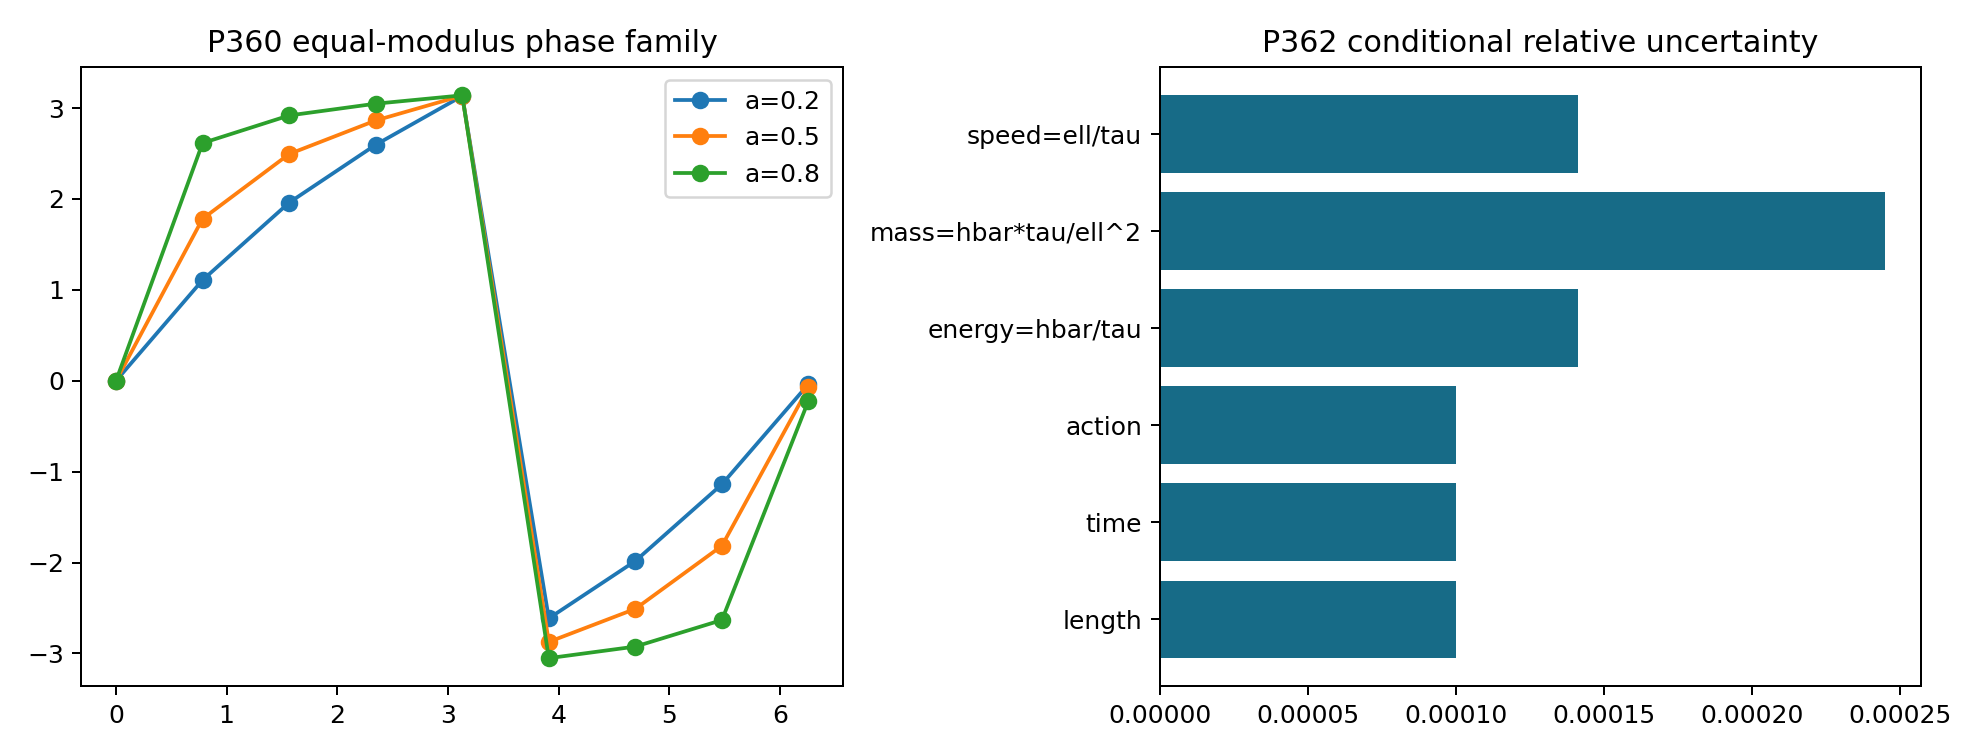
\includegraphics[width=0.97\textwidth]{FIN_Programs_351_364_Figures/p360_p362_phase_metrology.png}
\caption{Equal-modulus analytic inner-factor phases and conditional conversion-frame uncertainty.}
\end{figure}

\chapter{P363 --- FIN Operational Resource Completion}

\section{Objective}

The purpose of FORC is not to claim that FIN has become physical. It provides the smallest typed language in which the missing operational objects can be stated without conflating them with the strict operator.

\section{Axioms ranked by necessity}

\subsection{A1 --- typed spectral base}

There are distinct typed objects

\[
\mathsf K_{\mathrm{legacy}},
\qquad
\mathsf K_{\mathrm{strict}},
\]

with their declared carrier and provenance data.

\textbf{Necessity rank: 1.}

Removing A1 leaves a generic resource category that no longer refers to FIN and permits silent kernel substitution.

\subsection{A2 --- resource grading}

Each object carries a grade

\[
r\in\mathbb N^5.
\]

\textbf{Necessity rank: 2.}

Removing A2 makes the signed, phase, orientation, scale, and cross-law obstructions unexpressible.

\subsection{A3 --- resource-nonincreasing free morphisms}

A free morphism cannot increase any resource coordinate.

\textbf{Necessity rank: 3.}

Without A3, a free arrow from the zero object to a unit-resource object creates any missing bridge resource and destroys the obstruction theory.

\subsection{A4 --- additive monoidal composition}

Parallel composition adds grades.

\textbf{Necessity rank: 4.}

Removing A4 does not destroy single-object mathematics, but composition, cancellation, and catalysis become undefined.

\subsection{A5 --- operational realization functor}

A physical realization maps mathematical objects and morphisms to:

\begin{itemize}
\item 
states and preparations;

\item 
calibrated clocks;

\item 
channels or dynamical propagators;

\item 
environments;

\item 
instruments and apparatus settings;

\item 
outcome spaces and records;

\item 
probability laws;

\item 
independently frozen raw data.

\end{itemize}

\textbf{Necessity rank: 5 for mathematics, rank 1 for physics.}

A1--A4 define pure mathematics. A5 is the smallest bridge that makes an experimental proposition possible.

\section{Independence and removal tests}

\begin{center}
\begingroup\small
\setlength{\tabcolsep}{2.5pt}
\renewcommand{\arraystretch}{1.16}
\begin{longtable}{@{}p{0.146\textwidth}p{0.299\textwidth}p{0.415\textwidth}@{}}
\toprule
\textbf{Axiom removed} & \textbf{Surviving structure} & \textbf{Lost structure} \\
\midrule
\endhead
A1 & Abstract \(\mathbb N^5\) resource preorder & FIN kernel identity and split \\
A2 & Typed objects and arrows & Quantitative missing-resource accounting \\
A3 & Graded monoidal graph & No-free-generation meaning \\
A4 & Single-system resource preorder & Multi-system composition and no-catalysis theorem \\
A5 & Complete mathematical FORC category & Empirical interpretation and falsifiability \\
\bottomrule
\end{longtable}
\endgroup
\end{center}

Each remaining fragment has an explicit model, so no axiom is recovered merely from the others in the declared signature.

\section{Smallest physics bridge}

The minimal bridge is not one new scalar. It is:

\[
\boxed{
\text{FORC object}
\xrightarrow{\ \mathcal R\ }
(\text{preparation, clock, channel, environment,
instrument, apparatus, record})
}
\]

plus calibrated dimensional standards and independent custody.

This answers the recurring missing-object question: the operator alone defines many mathematical dynamics, but it does not choose which dynamics is performed, how time is calibrated, how a state is prepared, what constitutes an outcome, or what physical record tests the probability law.

\section{What FORC does not close}

FORC does not provide:

\begin{itemize}
\item 
the QW-2191 selector;

\item 
a strict internal orientation source;

\item 
a legacy-to-strict completion theorem;

\item 
a role-transfer theorem;

\item 
an internal dimensional source;

\item 
a laboratory realization;

\item 
a total physical action.

\end{itemize}

It is a controlled axiomatic completion of the language, not a proof of the missing physics.

\chapter{P364 --- certified physical reservoir gate}

A physical reservoir bundle would need:

\begin{itemize}
\item 
specified preparation maps;

\item 
calibrated interaction time;

\item 
a channel/\allowbreak{}process description;

\item 
environmental controls;

\item 
vertex-resolving or otherwise informationally complete instruments;

\item 
raw event-level records;

\item 
calibration hashes;

\item 
independent custody and unblinding.

\end{itemize}

No admitted bundle was found.

\textbf{[Blocked by external evidence]}

The strict heat semigroup

\[
P_t=e^{-tA}
\]

is a mathematical channel candidate. Code-generated samples from it are not evidence that a physical reservoir implements it.

\chapter{Newly constructed theoretical objects}

\begin{center}
\begingroup\small
\setlength{\tabcolsep}{2.5pt}
\renewcommand{\arraystretch}{1.16}
\begin{longtable}{@{}p{0.205\textwidth}p{0.224\textwidth}p{0.223\textwidth}p{0.208\textwidth}@{}}
\toprule
\textbf{Object} & \textbf{Definition} & \textbf{What it resolves} & \textbf{What it does not resolve} \\
\midrule
\endhead
O101 Envelope Krawczyk Cell & Rational box with \(\mathcal K(X)\subset\mathrm{int}(X)\) & Exact primal existence and local uniqueness & Physical meaning of signed mass \\
O102 Oscillatory Primal-Dual Interval & Exact dual Bernstein witness plus exact fixed-support interval measure & Theorem-grade \(\mathcal N_{\mathrm{osc}}\) enclosure & Selection of quantum/\allowbreak{}classical interpretation \\
O103 Refreeze Blind Contract & Custody-separated one-shot hold-out manifest & Defines admissible prediction evidence & Supplies no data \\
O104 Distance-Functor Naturality Boundary & Carrier category plus distance transport and defect & Exact scope of radial naturality & Legacy-to-strict completion \\
O105 Loss-Calibrated Photonic Transfer Tube & Family of conditional distributions under declared loss/\allowbreak{}noise & Synthetic apparatus robustness & Real hardware feasibility \\
O106 Perfect-Comb Collapse Certificate & Convex-zero parallel witness plus universal upper bound & Full adaptive optimum at saturation points & Subcritical comb optimum \\
O107 Anchored Clock Envelope & Maximum-gap minimax design after calibration & Sampling placement & Origin of time unit \\
O108 Cancellative Bridge-Resource Monoid & \((\mathbb N^5,+,\geq)\) & Complete monotones and no catalysis & Physical free-operation class \\
O109 Inner-Factor Phase Torsor & Analytic candidates modulo inner factors & Exact amplitude-phase nonuniqueness & Strict phase source \\
O110 Conversion Covariance Pushforward & \(A\Sigma A^\top\) for log-unit exponents & Uncertainty propagation & Dimensional standards \\
O111 FORC & Typed spectral/\allowbreak{}resource category plus realization functor & Missing operational language & Strict-core or empirical closure \\
O112 External Physical Admission Pair & Hardware and reservoir bundle contracts & Prevents synthetic-evidence substitution & Supplies no laboratory record \\
\bottomrule
\end{longtable}
\endgroup
\end{center}

\chapter{Falsification ledger}

\section{Surviving claims}

\begin{enumerate}
\item 
\textbf{\statusProven{}} The strict attenuation moment resource lies in the P351 enclosure.

\item 
\textbf{\statusProven{}} The strict oscillatory moment resource lies in the P352 enclosure.

\item 
\textbf{\statusProven{}} Radial graph kernels are natural under isomorphisms.

\item 
\textbf{\statusProven{}} They need not be natural under graph homomorphisms.

\item 
\textbf{\statusProven{}} A convex-zero parallel witness saturates the full-comb discrimination bound.

\item 
\textbf{\statusProven{}} Equispacing minimizes the declared maximum-gap clock bound.

\item 
\textbf{\statusProven{}} The additive five-resource preorder is complete and cancellative.

\item 
\textbf{\statusProven{}} Analytic inner factors obstruct amplitude-only phase reconstruction.

\item 
\textbf{\statusProven{}} Dimensional conversion covariance is a linear pushforward in logarithmic coordinates.

\item 
\textbf{\statusProven{}} A mathematical FORC model can exist without an operational realization.

\end{enumerate}

\section{Refuted claims}

\begin{enumerate}
\item 
\textbf{\statusRefuted{}} The P351 primal result is merely a floating root.

\item 
\textbf{\statusRefuted{}} The P352 continuum constraints are certified only by sampled grid points.

\item 
\textbf{\statusRefuted{}} A radial formula is automatically natural for arbitrary graph morphisms.

\item 
\textbf{\statusRefuted{}} Analyticity or causality plus amplitude uniquely determines the strict phase.

\item 
\textbf{\statusRefuted{}} The previous digital twin is itself a hardware validation.

\item 
\textbf{\statusRefuted{}} A resource category automatically supplies a physical realization.

\end{enumerate}

\section{Unresolved claims}

\begin{enumerate}
\item 
Exact interval certification of the four FIN convex-zero channel witnesses.

\item 
The subcritical unrestricted adaptive-comb curve.

\item 
A carrier-natural source-independent legacy-to-strict completion.

\item 
A physical free-operation semantics for the five resource coordinates.

\item 
A causal analytic coordinate and outer theorem derived from FIN.

\item 
Independent QW hold-out validation.

\item 
Calibrated photonic or reservoir realization.

\item 
Conditional electroweak blind testing.

\item 
External dimensional standards and their covariance.

\item 
Selector, role transfer, total action, Standard Model, gravity, or ToE closure.

\end{enumerate}

\chapter{Recommended Programs P365--P378}

The following programs are ranked by estimated probability of producing a scientifically useful result, not by probability of confirming FIN.

\begin{center}
\begingroup\small
\setlength{\tabcolsep}{2.5pt}
\renewcommand{\arraystretch}{1.16}
\begin{longtable}{@{}p{0.091\textwidth}p{0.276\textwidth}p{0.321\textwidth}p{0.171\textwidth}@{}}
\toprule
\textbf{Program} & \textbf{Research question} & \textbf{Primary deliverable} & \textbf{Probability of useful result} \\
\midrule
\endhead
P365 & Can the P351/\allowbreak{}P352 rational certificates be independently kernel-checked? & Lean/\allowbreak{}Coq certificate checker for interval, Bernstein, and Vandermonde steps & 0.90 \\
P366 & Can the P352 enclosure be narrowed by exact alternation? & Rational Remez/\allowbreak{}semidefinite dual and optimized certified support & 0.80 \\
P367 & Does the QW candidate survive a truly independent frozen hold-out? & Custody-separated one-shot external validation & 0.55 \\
P368 & What is the largest graph-morphism category supporting strict radial naturality? & Classification theorem for distance-preserving/\allowbreak{}enriched morphisms & 0.80 \\
P369 & Do component-level correlated losses destroy the mesh tube? & Identifiable per-coupler loss/\allowbreak{}phase digital twin and calibration theorem & 0.75 \\
P370 & Can a twelve-mode device realize the declared transfer matrix? & Calibrated photonic pilot with raw event-level data & 0.45 \\
P371 & Does adaptivity improve discrimination below the perfect-witness time? & Full subcritical quantum-comb SDP with primal-dual certificates & 0.65 \\
P372 & Can the bounded-curvature clock design be externally anchored? & Traceable clock calibration and preregistered interpolation test & 0.55 \\
P373 & Which physical channels realize the O108 free morphisms? & Operational semantics or a no-go theorem for each resource coordinate & 0.65 \\
P374 & Can any FIN-derived causal analytic extension be outer? & Inner/\allowbreak{}outer factor classification and phase comparison & 0.55 \\
P375 & Does the conditional P348 electroweak vector survive a blind test? & One-shot preregistered external sector test & 0.25 \\
P376 & Can \((\ell_*,\tau_*,\hbar_*)\) be calibrated with a full covariance record? & Standards manifest and propagated uncertainty budget & 0.50 \\
P377 & Is FORC universal among typed operational completions satisfying A1--A5? & Initiality/\allowbreak{}universality theorem or counterexample & 0.70 \\
P378 & Can a controlled open system implement the strict heat semigroup? & Reservoir-engineering experiment with process tomography & 0.35 \\
\bottomrule
\end{longtable}
\endgroup
\end{center}

\section{P365 --- kernel-checked exact certificates}

Translate:

\begin{itemize}
\item 
the rational interval operations;

\item 
the Krawczyk inclusion;

\item 
the fifth-root integer inequalities;

\item 
the Taylor remainder;

\item 
the Bernstein bounds;

\item 
the Vandermonde identity;

\end{itemize}

into a proof assistant with arbitrary-precision integer reflection.

\textbf{Success criterion:} a small independent checker accepts a compact certificate without executing the discovery code.

\textbf{Failure value:} identification of any hidden assumption in the exact arithmetic pipeline.

\section{P366 --- exact oscillatory alternation}

The P352 gap is approximately \(8.17\times10^{-5}\). Search for:

\begin{itemize}
\item 
an alternation-certified extremal dual;

\item 
a better rational support;

\item 
a moment semidefinite hierarchy with exact rational recovery;

\item 
an interval proof that primal and dual contact sets coincide.

\end{itemize}

\textbf{Success criterion:} theorem-grade width below \(10^{-7}\).

\section{P367 --- independent QW hold-out}

This is not a coding program. It requires:

\begin{enumerate}
\item 
frozen prediction hash;

\item 
independently controlled data;

\item 
distinct provider, registrar, and analyst;

\item 
one unblinding;

\item 
publication of failure without parameter repair.

\end{enumerate}

\section{P368 --- enriched graph naturality}

Classify the maximal morphism class \(\mathcal C\) for which

\[
K_H\circ(f\times f)=K_G
\]

holds. Candidate classes include:

\begin{itemize}
\item 
graph isomorphisms;

\item 
isometric embeddings;

\item 
distance-regular coverings with fiber normalization;

\item 
metric correspondences with a controlled defect;

\item 
enriched functors carrying distance as explicit data.

\end{itemize}

The program must test both strict and legacy kernels without identifying them.

\section{P369 --- component-level photonic identifiability}

Replace output-diagonal loss by:

\begin{itemize}
\item 
loss at every Givens element;

\item 
correlated phase drift;

\item 
unknown splitter ratios;

\item 
detector confusion and dark counts;

\item 
temporal source impurity.

\end{itemize}

Determine which parameters are identifiable from basis, plus, and phase-shifted probes.

\section{P370 --- photonic pilot}

Implement a reduced or full twelve-mode device. Required outputs are raw timestamped detection events and independent calibration records, not a rendered interference image.

\section{P371 --- subcritical adaptive comb}

Construct the full causal comb SDP. For every sampled time report:

\begin{itemize}
\item 
primal strategy;

\item 
dual upper certificate;

\item 
gap;

\item 
memory dimension;

\item 
whether adaptivity improves over the parallel optimum.

\end{itemize}

No conclusion should be drawn from solver output without a dual residual and conditioning audit.

\section{P372 --- calibrated clock test}

Use a traceable reference to anchor \(\tau\). Test whether the bounded-curvature class is empirically adequate before applying the equispaced theorem.

\section{P373 --- operational semantics of resources}

For each O108 coordinate, define:

\begin{itemize}
\item 
physical objects carrying the resource;

\item 
free operations;

\item 
observable monotones;

\item 
composition;

\item 
discard maps;

\item 
conversion experiments.

\end{itemize}

If no such interpretation exists, prove the obstruction rather than keeping the coordinate as physics.

\section{P374 --- causal analytic extension}

Search for a source-derived variable \(z\) or \(\omega\) in which the strict kernel becomes boundary data of an analytic transfer function. Then:

\begin{itemize}
\item 
factor the function into inner and outer parts;

\item 
test zero locations;

\item 
compare reconstructed and frozen phases;

\item 
quantify the extra axioms.

\end{itemize}

\section{P375 --- conditional electroweak blind test}

This program remains low probability because the sector map is conditional. It is nevertheless useful as a falsification exercise if assumptions and data are frozen before inspection.

\section{P376 --- dimensional standards package}

Supply independent calibrated estimates of \((\ell_*,\tau_*,\hbar_*)\), their covariance, traceability, and stability. The output is a conversion frame, not a claim that FIN generated SI units.

\section{P377 --- FORC universality}

Formulate a category of operational completions satisfying A1--A5 and test whether FORC is initial, free, or merely one model. A counterexample is as valuable as a positive universal property.

\section{P378 --- reservoir implementation}

Engineer a controlled open system approximating

\[
\rho\mapsto\mathcal E_t(\rho)
\]

whose vertex populations agree with the strict heat semigroup under declared preparations and instruments. Perform process tomography and compare homogeneous-semigroup versus non-Markovian alternatives.

\section{Recommended execution order}

\[
\boxed{
\mathrm{P365}
\rightarrow
\mathrm{P366}
\rightarrow
\mathrm{P368}
\rightarrow
\mathrm{P371}
\rightarrow
\mathrm{P373}
}
\]

This order first hardens the new theorems, then clarifies carrier and operational structure, and only then spends substantial effort on external apparatus.

\chapter{Present state of the theory}

\section{What the strict operator currently generates}

Given a self-adjoint positive semidefinite generator \(A\), functional calculus yields:

\[
U_t=e^{-itA},
\qquad
P_t=e^{-tA},
\qquad
G_z=(A+zI)^{-1},
\]

as well as spectral measures and variational quadratic forms. This unifies wave, diffusion, and resolvent mathematics.

The same operator does not select:

\begin{itemize}
\item 
whether a laboratory uses \(U_t\), \(P_t\), or another channel;

\item 
the prepared input state;

\item 
the time unit;

\item 
the environment;

\item 
the instrument;

\item 
the recorded outcome;

\item 
the observer's operational role.

\end{itemize}

That distinction remains the central barrier between operator mathematics and physics.

\section{What the signed resources add}

The P351/\allowbreak{}P352 quantities rigorously measure the failure of selected finite sequences to admit positive scalar path representations on \([0,1]\). The phase-bearing sequence requires a larger signed resource than the attenuation envelope.

This is a real mathematical distinction. It is not yet a physical mechanism.

\section{What naturality adds}

P354 shows that the strict formula is invariant under relabeling but not under arbitrary coarse graph maps. Carrier choice is therefore not mathematically invisible. A genuine universal completion law must declare its morphisms.

\section{What FORC adds}

FORC converts a vague list of missing notions into a typed interface:

\[
\text{spectral object}
+\text{resources}
+\text{realization functor}.
\]

The realization functor is not internally derived. This is not a defect of formalism; it is the precise location where empirical physics must enter.

\chapter{Final conclusion}

The deepest result of this round is not a new cosmological claim. It is a sharper separation theorem.

The FIN strict kernel supports a coherent and increasingly certifiable operator theory. Its attenuation and oscillatory sequences possess exact signed-moment resource enclosures. Its radial construction is functorial on the correct carrier groupoid. Its wave dynamics admits explicit multi-use discrimination witnesses. Its clock and metrology problems can be stated as clean minimax and covariance problems. Its amplitude cannot determine its phase without an extra analytic selection axiom.

What remains missing is not another function of \(A\). The missing object is an operational realization:

\[
\boxed{
\mathcal R:
\text{typed FIN mathematics}
\longrightarrow
\mathsf{OperationalModel}
}
\]

Here \(\mathsf{OperationalModel}\) contains calibrated preparations, dynamics, clocks, environments, instruments, apparatus, and records.

No theorem of the spectral calculus can create \(\mathcal R\) from a dimensionless operator alone. FORC makes that impossibility explicit while showing exactly what additional axioms and external evidence would suffice to formulate a physical test.

Therefore the present strongest defensible interpretation is:

\begin{quote}\itshape
FIN is a dimensionless typed spectral-operator and signed-resource framework with conditional operational completions. It is not yet a physical theory, because no independently calibrated realization functor has been supplied.

\end{quote}

This conclusion survives every falsification attempt executed in P351--P364.

\chapter{Reproducibility}

Run:

\begin{itemize}
\item 
MPLCONFIGDIR=/\allowbreak{}tmp/\allowbreak{}mpl-fin-1031 python3 fin\_programs\_351\_364.py

\item 
MPLCONFIGDIR=/\allowbreak{}tmp/\allowbreak{}mpl-fin-1031 python3 -m unittest -v test\_fin\_programs\_351\_364.py

\end{itemize}

Expected result: 16 tests passed, 0 failed. The dependency-free Lean 4.28 structural core must compile.

The primary machine-readable artifacts are:

\begin{itemize}
\item 
FIN\_Programs\_351\_364\_Results.json;

\item 
fourteen CSV audit tables;

\item 
FIN\_Programs\_351\_364\_Formal\_Core.lean;

\item 
four figures;

\item 
the source program and regression suite.

\end{itemize}

\chapter{Suggested citation}

\.Zuchowski, K. (2026). \emph{FIN Research Programs P351--P364: Rigorous Moment Certificates, Graph Naturality, Operational Resource Completion, and External Physics Gates} (Release 10.31; Version 1.0.0) [Preprint]. Zenodo.


\clearpage
\chapter*{Reproduction certificate}
\addcontentsline{toc}{chapter}{Reproduction certificate}
\begin{Verbatim}[fontsize=\small]
MPLCONFIGDIR=/tmp/mpl-fin-1031 \
python3 fin_programs_351_364.py

MPLCONFIGDIR=/tmp/mpl-fin-1031 \
python3 -m unittest -v test_fin_programs_351_364.py
\end{Verbatim}
Expected result: 16 tests passed, 0 failed. The dependency-free Lean 4.28
structural core must compile. P353, P356, P361, and P364 remain external
admission gates; no synthetic record is accepted as laboratory evidence.

\medskip
\noindent\textbf{Suggested citation:}

\.Zuchowski, K. (2026). \emph{FIN Research Programs P351--P364:
Rigorous Moment Certificates, Graph Naturality, Operational Resource
Completion, and External Physics Gates} (Release 10.31; Version 1.0.0)
[Preprint]. Zenodo.

\end{document}
